\documentclass[12pt]{standalone}
\usepackage[english]{babel}
\usepackage[utf8]{inputenc}

\usepackage{comment}
\usepackage{amsmath}
\usepackage{tikz}
\usepackage{circuitikz} % for circuits!
\usetikzlibrary{arrows.meta} % for loads
\usepackage{float}
\usetikzlibrary{positioning}
\usetikzlibrary{calc}

\begin{document}
	
	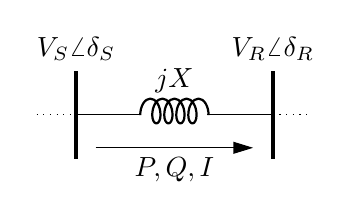
\begin{tikzpicture}[american voltages,
	scale=.7, 
	breaker/.style={rectangle,draw=black,fill=white},
	load/.style={-{Triangle[length=3.5mm,width=2.5mm,open,fill=black]}},
	node distance = 1.5 cm and 1.5cm]
	
	% coordinate def
	\coordinate (start) at (0,0) {};
	\coordinate[right = .5cm of start] (sendingBus) {};
	\coordinate[right = 2.5 of sendingBus] (recBus) {};
	\coordinate[right = .5cm of recBus] (end) {};
	
	% bus lines
	\draw[ultra thick] ([yshift=-0.8cm]sendingBus.south) -- ([yshift=+0.8cm]sendingBus.north);
	\draw[ultra thick] ([yshift=-0.8cm]recBus.south) -- ([yshift=+0.8cm]recBus.north);
	
	% connecting lines
	\draw[dotted] (start) -- (sendingBus);
	\draw[dotted] (recBus) -- (end);
	\draw (sendingBus) to [L, l=$jX$] (recBus);
	
	% Bus voltage labels
	\draw ($(sendingBus) +(0,+1.2)$) node {$V_S \angle \delta_S$};
	\draw ($(recBus) +(0,+1.2)$) node {$V_R \angle \delta_R$};
	
	% Power Flow Line
	\draw[-{Triangle[length=2.5mm,width=1.5mm,open,fill=black]}] ($(sendingBus)!0.1!(recBus)+(0,-.6)$) -- ($(sendingBus)!0.9!(recBus)+(0,-.6)$);
	
	% Power Flow Label
	\draw ($(sendingBus)!0.5!(recBus)+(0,-1.)$) node {$P,Q,I$};
	\end{tikzpicture}
	
\end{document}